% !TEX program = xelatex
% !TeX spellcheck = ru_RU_yo

\documentclass[xetex,t]{beamer}

\usepackage{xecyr}
\usepackage{xunicode}
\usepackage{fontspec}
\defaultfontfeatures{Ligatures=TeX}
\setmainfont{ALS Schlange sans}

\usepackage{polyglossia}
\setdefaultlanguage[spelling=modern]{russian}
\newfontfamily{\cyrillicfont}{ALSSchlangesans}
\newfontfamily{\cyrillicfontsf}{ALSSchlangesans}
\newfontfamily{\cyrillicfonttt}{Droid Sans Mono}

\usepackage[euler-digits,small]{eulervm}
\AtBeginDocument{\renewcommand{\hbar}{\hslash}}

\definecolor{ifmoblue}{RGB}{25,70,186}
\definecolor{ifmored}{RGB}{236,11,67}

\setbeamertemplate{itemize items}[circle]

\usepackage{epstopdf}
\usepackage{graphicx}
\usepackage{amsmath}
\usepackage{nicefrac}
\usepackage{ctable}
\usepackage{ragged2e}

\usepackage{pifont}
\newcommand{\cmark}{\ding{51}}%
\newcommand{\xmark}{\ding{55}}%


\usepackage{xcolor}
\newcommand{\highlight}[1]{\colorbox{orange!50}{$\displaystyle#1$}}

\usepackage{tikz}
\usetikzlibrary{calc, shadings, shadows, positioning, shapes.arrows, backgrounds}

\tikzset{
  zigzag/.style={to path={ -- ($(\tikztostart)!.51!-3:(\tikztotarget)$) -- ($(\tikztostart)!.49!3:(\tikztotarget)$) -- (\tikztotarget) \tikztonodes}},
  new dashed/.style={dash pattern=on 8pt off 4pt}
}

\newcommand{\email}[1]{{\scriptsize\texttt{#1}}}

\usebackgroundtemplate{}

\titlegraphic{
\includegraphics[width=5cm]{ifmo/logo-blue}}
\title{Разработка веб-приложения для работы\\с программным пакетом высокоточного позиционирования RTKLIB}
\author[Кузнецов А.А., P3410]{Кузнецов Андрей Андреевич, ФПИиКТ, ИПМ, Р4215}
\date[]{Научный руководитель: Соснин В.В., к.т.н., доцент}

\usetheme{ifmo}
\setbeamersize{text margin left=0.6cm,text margin right=0.5cm}

\begin{document}

%
% Title
%
\begin{frame}
  \titlepage
\end{frame}


%
% DGPS
%
\begin{frame}
  \frametitle{Дифференциальная GPS}

  \only<1>{
    \begin{center}
      \textbf{Дифференциальная GPS} (англ. \emph{Differential Global Positioning System}) -- система, предназначенная для повышения точности сигналов GPS. Принцип работы данной системы заключается в~измерении и~учёте разницы между рассчитанной и~закодированной псевдодальностями до спутников.
    \end{center}
    
    \vskip -0.25cm
    
    \begin{figure}[h]
      \centering
      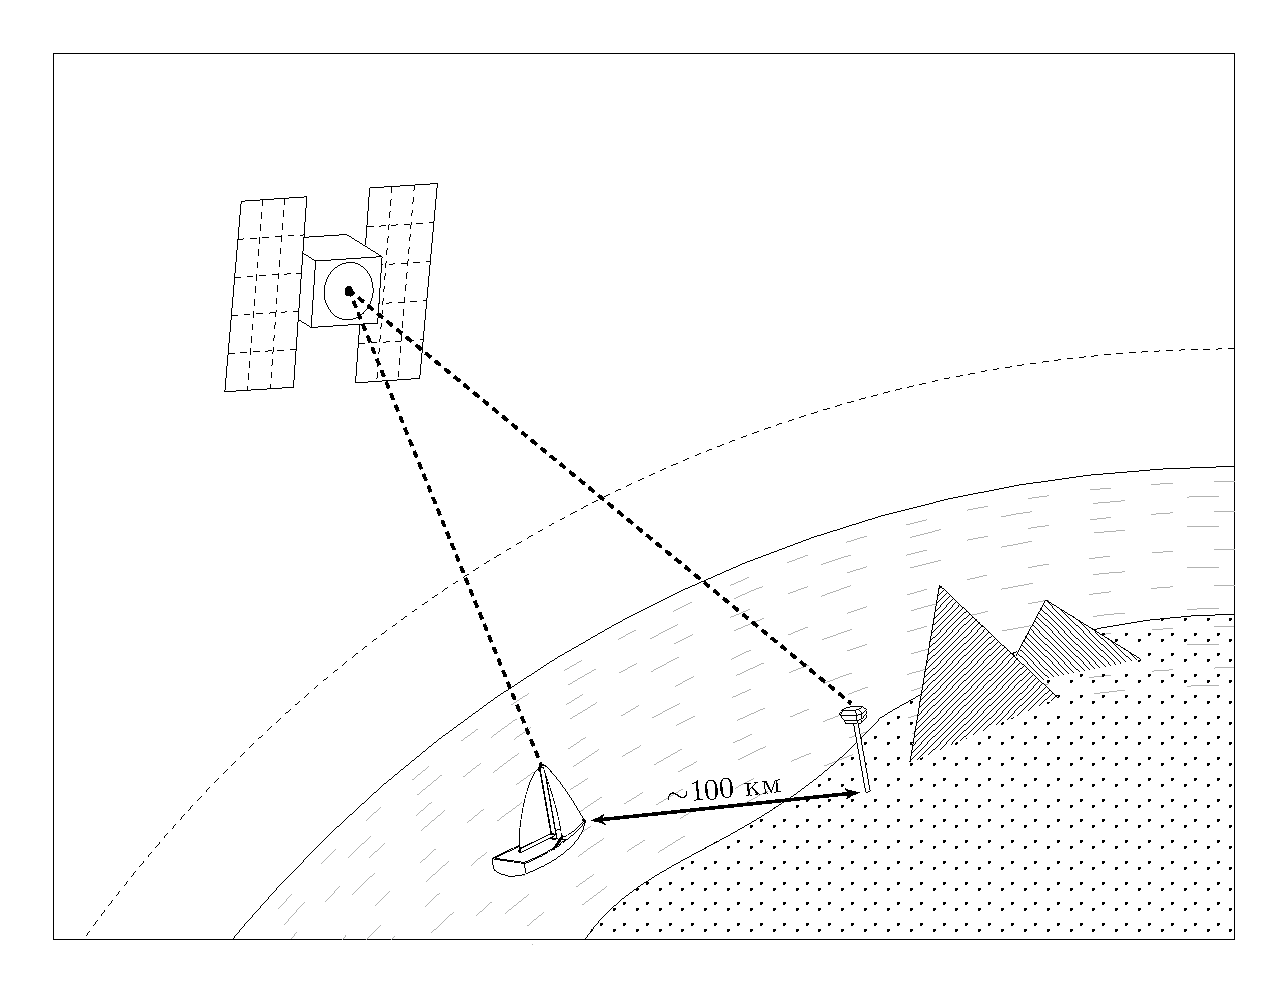
\includegraphics[height=4.5cm]{../img/tikz/dgps-one/pic}
    \end{figure}
  }

  \only<2>{
    \begin{figure}[t]
      \centering
      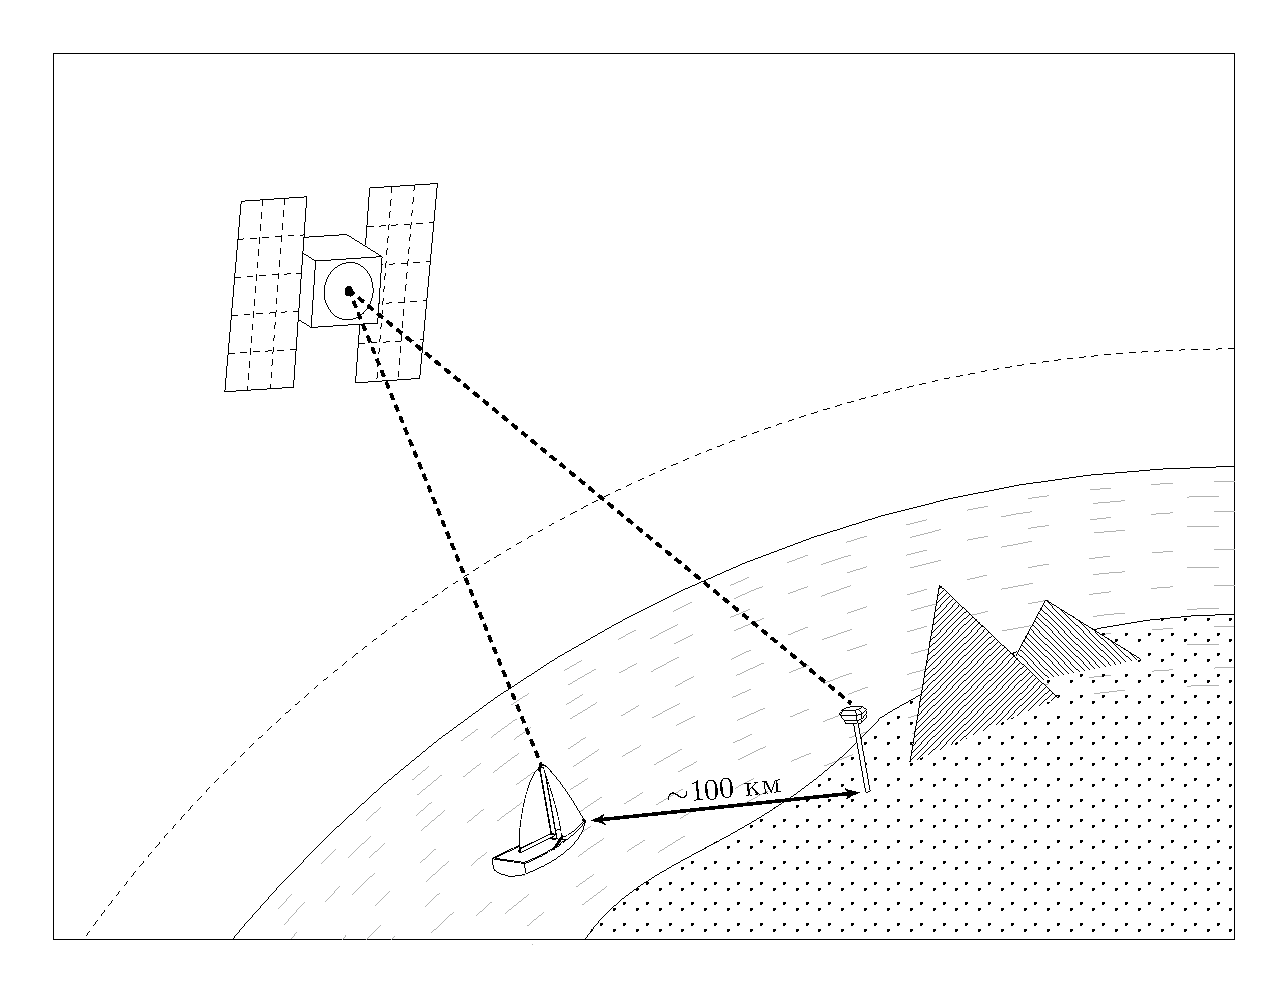
\includegraphics[height=7.25cm]{../img/tikz/dgps-one/pic}
    \end{figure}
  }
\end{frame}


%
% RTK
%
\begin{frame}
  \frametitle{Кинематика реального времени}

  \begin{center}
    \textbf{Кинематика реального времени} (англ. \emph{Real Time Kinematic, RTK}) -- режим работы, при котором приём и~применение поправок с~базы происходят в~реальном времени, что позволяет получать результат практически сразу. Важнейшей особенностью данного режима является тот факт, что для обеспечения работы необходима постоянная связь между ровером и~базой.
  \end{center}

  \vskip 0.25cm

  \only<2>{
    \begin{minipage}{\textwidth}
      \centering
      \begin{minipage}[t]{.3\textwidth}
        \centering
        \begin{figure}[h]
          \centering
          
\includegraphics[height=18pt]{../img/trimble}
        \end{figure}
        от \$2495

        {
          \scriptsize
          \color{gray}{Trimble R1 GNSS Receiver}
        }
      \end{minipage}
      \hspace{1em}
      \begin{minipage}[t]{.3\textwidth}
        \centering
        \begin{figure}[h]
          \centering
          
\includegraphics[height=17pt]{../img/javad}
        \end{figure}
        от \$2490

        {
          \scriptsize
          \color{gray}{TRIUMPH-2}
        }
      \end{minipage}
    \end{minipage}
  }
\end{frame}


%
% RTKLIB
%
\begin{frame}
  \frametitle{RTKLIB}
  
  \begin{center}
    \textbf{RTKLIB} -- программный пакет с~открытым исходным кодом, предназначенный для осуществления стандартного и~высокоточного позиционирования с~помощью глобальных навигационных спутниковых систем.
  \end{center}
  
  \begin{figure}[h]
    \centering
    
\includegraphics[height=2cm]{../img/rtklib}
  \end{figure}
\end{frame}


%
% RTKLIB problems
%
\begin{frame}
  \frametitle{RTKLIB}
  \framesubtitle{Проблемы использования}

  \begin{figure}[h]
    \centering
    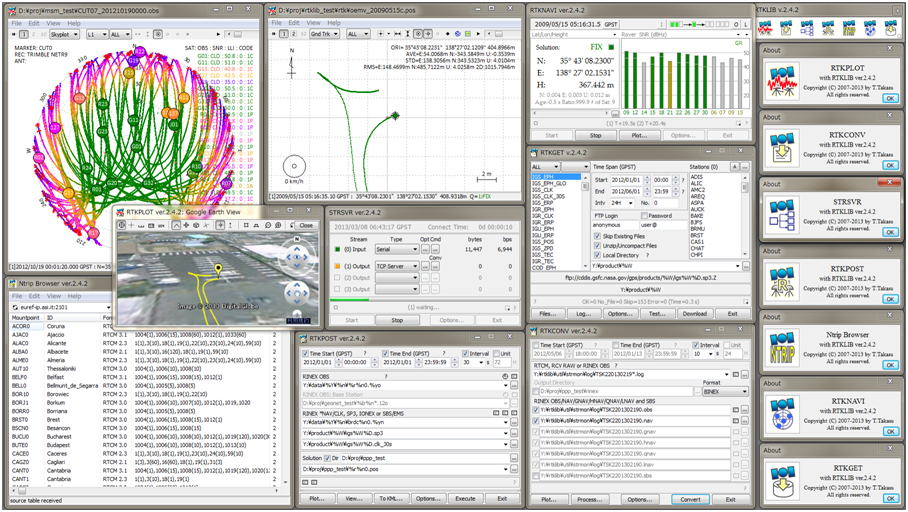
\includegraphics[width=.95\textwidth]{../img/rtklib-hell}
  \end{figure}
\end{frame}


%
% Main task
%
\begin{frame}
  \frametitle{Характеристика проведённой работы}
  
  \textbf{Предмет исследования} -- ...
  \vskip .75cm
  \textbf{Цель работы} -- ...
\end{frame}


%
% Receivers review
%
\begin{frame}
    \frametitle{Обзор существующих решений}
    \framesubtitle{Интерфейсы для управления приёмниками}
\end{frame}


%
% Web apps review
%
\begin{frame}
  \frametitle{Обзор существующих решений}
  \framesubtitle{Веб-интерфейсы для управления устройствами}
\end{frame}


%
% Reach & Reach~RS
%
\begin{frame}
  \frametitle{Платформа для разработки}
\end{frame}


%
% Required features
%
\begin{frame}
  \frametitle{Требования к функциональности веб-приложения}
\end{frame}


%
% Raw architecture
%
\begin{frame}
  \frametitle{Общая архитектура приложения}
\end{frame}


%
% Tools
%
\begin{frame}
  \frametitle{Средства разработки}
\end{frame}


%
% System architecture
%
\begin{frame}
  \frametitle{Общая архитектура приложения}
  \vskip -0.75cm
  \begin{figure}[h]
    \centering
    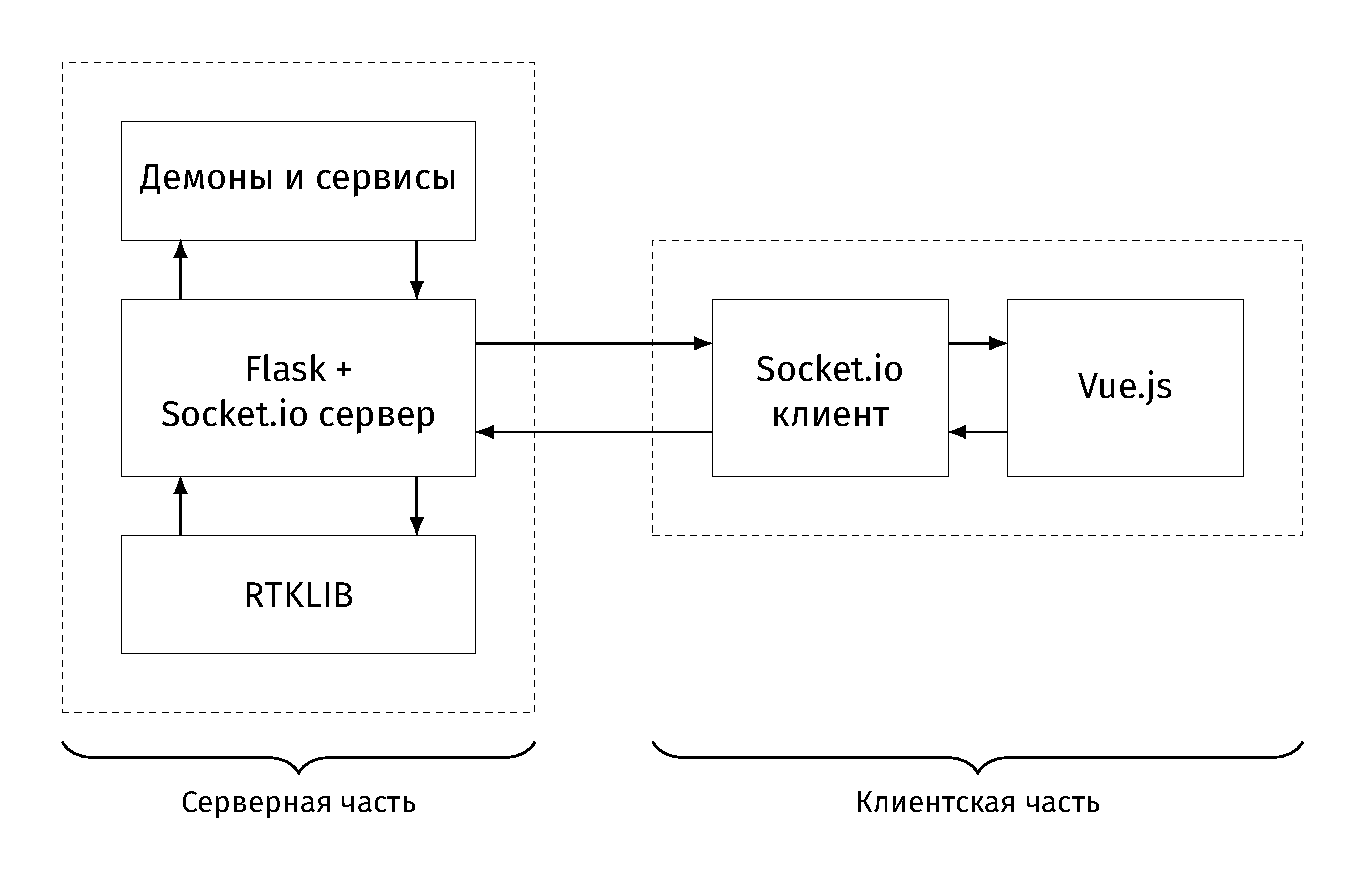
\includegraphics[width=.95\textwidth]{../img/tikz/system-architecture/pic_sans_no-border}
  \end{figure}
\end{frame}


%
% FE architecture
%
\begin{frame}
  \frametitle{Архитектура клиентской части приложения}
\end{frame}


%
% Responsive UI
%
\begin{frame}
  \frametitle{Разработка веб-приложения}
  \framesubtitle{Адаптивный интерфейс}
\end{frame}


%
% Tabs
%
\begin{frame}
  \frametitle{Разработка веб-приложения}
  \framesubtitle{Разделение на интерфейса на секции}
\end{frame}


%
% Testing
%
\begin{frame}
  \frametitle{Тестирование приложения}
\end{frame}


%
% Results
%
\begin{frame}
  \frametitle{Результаты}
\end{frame}


%
% The End
%
\begin{frame}[c]
\begin{center}
  \Huge\bfseries
  \color{ifmoblue}{Спасибо за внимание}
\end{center}
\end{frame}

\end{document}
